\documentclass[a4paper,12pt]{article}

\usepackage[utf8]{inputenc}
\usepackage[T1]{polski}
\usepackage{helvet}
\usepackage{graphicx}
\usepackage{color}
\usepackage{geometry}

\usepackage[unicode]{hyperref}
\usepackage{amsmath}
\usepackage{gensymb}
\usepackage{multirow}
\usepackage{multicol}
\usepackage{ amssymb }

\usepackage{lipsum} 
\usepackage{indentfirst}
\usepackage{tabularx}

\usepackage{listings}
\usepackage{color}

\definecolor{dkgreen}{rgb}{0,0.6,0}
\definecolor{gray}{rgb}{0.5,0.5,0.5}
\definecolor{mauve}{rgb}{0.58,0,0.82}
\lstset{frame=tb,
  language=python,
  aboveskip=3mm,
  belowskip=3mm,
  showstringspaces=false,
  columns=flexible,
  basicstyle={\small\ttfamily},
  numbers=none,
  numberstyle=\tiny\color{gray},
  keywordstyle=\color{blue},
  commentstyle=\color{dkgreen},
  stringstyle=\color{mauve},
  breaklines=true,
  breakatwhitespace=true,
  tabsize=2,
  basicstyle=\footnotesize
}

\usepackage{float}

\floatstyle{ruled}
\newfloat{kod}{htp}{lop}
\floatname{kod}{Kod}


%interrupt service routine
%gui , ui

\author{Wojciech Surówka}

\graphicspath{{fig/} {./fig/wykresy/} {./fig/schematy/} {./fig/zdjecia/}}
\geometry{hmargin={2cm, 2cm}, height=10.0in}

\begin{document}

% =====  STRONA TYTULOWA PRACY MAGISTERSKIEJKIEJ ====
% ostatnia modyfikacja: 2009/07/01, K. Malarz

\thispagestyle{empty}
%% ------------------------ NAGLOWEK STRONY ---------------------------------

\includegraphics[height=37.5mm]{agh_nzw_a_pl_1w_wbr}\\
\rule{30mm}{0pt}
{\large \textsf{Wydział Fizyki i Informatyki Stosowanej}}\\
\rule{\textwidth}{3pt}\\
\rule[2ex]
{\textwidth}{1pt}\\
\vspace{7ex}
\begin{center}
{\LARGE \bf \textsf{Praca magisterska}}\\
\vspace{13ex}
% --------------------------- IMIE I NAZWISKO -------------------------------
{\bf \Large \textsf{Wojciech Surówka}}\\
\vspace{3ex}
{\sf\small kierunek studiów:} {\bf\small \textsf{Fizyka Medyczna}}\\
\vspace{1.5ex}
{\sf\small specjalność:} {\bf\small \textsf{Techniki obrazowania i biometria}}\\
\vspace{10ex}
%% ------------------------ TYTUL PRACY --------------------------------------
{\bf \huge \textsf{System akwizycji danych pomiarowych dla szybkiego wielokanałowego układu scalonego o architekturze całkująco-zliczającej z detektorem promieniowania X}}\\
\vspace{14ex}
%% ------------------------ OPIEKUN PRACY ------------------------------------
{\Large Opiekun: \bf \textsf{dr inż. Piotr Wiącek}}\\
\vspace{16ex}
{\large \bf \textsf{Kraków, czerwiec 2020}}
\end{center}
%% =====  STRONA TYTUŁOWA PRACY MAGISTERSKIEJKIEJ ====

\newpage

%% =====  TYŁ STRONY TYTUŁOWEJ PRACY MAGISTERSKIEJKIEJ ====
\begin{center}
        {\bf\large\textsf{Oświadczenie studenta}}
\end{center}


{\sf Uprzedzony(-a) o odpowiedzialności karnej na podstawie art. 115 ust. 1 i 2 ustawy z dnia 4 lutego 1994 r. o prawie autorskim i prawach pokrewnych (t.j. Dz. U. z 2018 r. poz. 1191 z późn. zm.): ,,Kto przywłaszcza sobie autorstwo albo wprowadza w błąd co do autorstwa całości lub części cudzego utworu albo artystycznego wykonania, podlega grzywnie, karze ograniczenia wolności albo pozbawienia wolności do lat 3. Tej samej karze podlega, kto rozpowszechnia bez podania nazwiska lub pseudonimu twórcy cudzy utwór w wersji oryginalnej albo w postaci opracowania, artystyczne wykonanie albo publicznie zniekształca taki utwór, artystyczne wykonanie, fonogram, wideogram lub nadanie.'', a także uprzedzony(-a) o odpowiedzialności dyscyplinarnej na podstawie art. 307 ust. 1 ustawy z dnia 20 lipca 2018 r. Prawo o szkolnictwie wyższym i nauce (Dz. U. z 2018 r. poz. 1668 z późn. zm.) ,,Student podlega odpowiedzialności dyscyplinarnej za naruszenie przepisów obowiązujących w~uczelni oraz za czyn uchybiający godności studenta.'', oświadczam, że niniejszą pracę dyplomową wykonałem(-am) osobiście i samodzielnie i nie korzystałem(-am) ze źródeł innych niż wymienione w pracy.

\bigskip

Jednocześnie Uczelnia informuje, że zgodnie z art. 15a ww. ustawy o prawie autorskim i prawach pokrewnych Uczelni przysługuje pierwszeństwo w opublikowaniu pracy dyplomowej studenta. Jeżeli Uczelnia nie opublikowała pracy dyplomowej w terminie 6 miesięcy od dnia jej obrony, autor może ją opublikować, chyba że praca jest częścią utworu zbiorowego. Ponadto Uczelnia jako podmiot, o którym mowa w art. 7 ust. 1 pkt 1 ustawy z dnia 20 lipca 2018 r. --- Prawo o szkolnictwie wyższym i nauce (Dz. U. z 2018 r. poz. 1668 z późn. zm.), może korzystać bez wynagrodzenia i bez konieczności uzyskania zgody autora z utworu stworzonego przez studenta w wyniku wykonywania obowiązków związanych z odbywaniem studiów, udostępniać utwór ministrowi właściwemu do spraw szkolnictwa wyższego i~nauki oraz korzystać z utworów znajdujących się w prowadzonych przez niego bazach danych, w celu sprawdzania z wykorzystaniem systemu anty plagiatowego. Minister właściwy do spraw szkolnictwa wyższego i nauki może korzystać z prac dyplomowych znajdujących się w prowadzonych przez niego bazach danych w zakresie niezbędnym do zapewnienia prawidłowego utrzymania i rozwoju tych baz oraz współpracujących z nimi systemów informatycznych.}


\vspace{14ex}

\begin{center}
\begin{tabular}{lr}
~~~~~~~~~~~~~~~~~~~~~~~~~~~~~~~~~~~~~~~~~~~~~~~~~~~~~~~~~~~~~~~~~ &
................................................................. \\
~ & {\sf (czytelny podpis)}\\
\end{tabular}
\end{center}

%% =====  TYL STRONY TYTULOWEJ PRACY MAGISTERSKIEJKIEJ ====

\newpage
\rightline{Kraków, ?? czerwca 2020}
\begin{center}
{\bf Tematyka pracy magisterskiej i praktyki dyplomowej
Wojciecha Surówki,
studenta drugiego roku studiów drugiego stopnia na kierunku fizyka medyczna, specjalności Techniki obrazowania i biometria}\\
\end{center}

Temat pracy magisterskiej:
{\bf System akwizycji danych pomiarowych dla szybkiego wielokanałowego układu scalonego o architekturze całkująco-zliczającej z detektorem promieniowania X}\\

\begin{tabular}{rl}

Opiekun pracy:                  & dr inż. Piotr Wiącek\\
Recenzenci pracy:               & dr hab. inż. Owaki Śmaki\\
Miejsce praktyki dyplomowej:    & WFiIS AGH, Kraków\\
\end{tabular}

\begin{center}
{\bf Program pracy magisterskiej i praktyki dyplomowej}
\end{center}

\begin{enumerate}
\item Omówienie realizacji pracy magisterskiej z opiekunem.
\item Zebranie i opracowanie literatury dotyczącej tematu pracy.
\item Praktyka dyplomowa:
\begin{itemize}
\item zapoznanie się z ideą...,
\item uczestnictwo w eksperymentach/przygotowanie oprogramowania...,
\item dyskusja i analiza wyników...
\item sporządzenie sprawozdania z praktyki.
\end{itemize}
\item Kontynuacja obliczeń związanych z tematem pracy magisterskiej.
\item Zebranie i opracowanie wyników obliczeń.
\item Analiza wyników obliczeń numerycznych, ich omówienie i zatwierdzenie przez opiekuna.
\item Opracowanie redakcyjne pracy.
\end{enumerate}


\noindent
Termin oddania w dziekanacie: ?? czerwca 20??\\[1cm]

\begin{center}
\begin{tabular}{lcr}
.............................................................. & ~~~ &
.............................................................. \\
(podpis kierownika katedry) & & (podpis opiekuna) \\
\end{tabular}
\end{center}

\newpage

\noindent
Na kolejnych dwóch stronach proszę dołączyć kolejno recenzje pracy popełnione przez Opiekuna oraz Recenzenta (wydrukowane z systemu MISIO i podpisane przez odpowiednio Opiekuna i Recenzenta pracy). Papierową wersję pracy (zawierającą podpisane recenzje) proszę złożyć w dziekanacie celem rejestracji co najmniej na tydzień przed planowaną obroną.

\linespread{1.3}
\selectfont

\newpage
\linespread{1.3}
\selectfont
\tableofcontents
\newpage


\section{Wprowadzenie}
\subsection{Cel pracy}

Celem pracy było zaprojektowanie i skonstruowanie układu wspierającego system detekcji promieniowania X: RXHDR\_V2 \cite{master}.\\
Cele szczegółowe:
\begin{itemize}
        \item Szesnasto-kanałowy odczyt i zliczenie impulsów o częstotliwości osiągającej do 2.5$\frac{MHz}{kanal}$ z wykorzystaniem mikrokontrolera \textit{Arduiono Due}.
        \item Stworzenie oprogramowania pozwalającego na komunikację pomiędzy mikrokontrolerem a komputerem wspierającym. 
        \item Wizualizacja i archiwizacja uzyskanych danych. 
\end{itemize}

\subsection{Wstęp teoretyczny}

W celu stworzenia programu dla tego projektu konieczne jest zrozumienie niskopoziomowego i wysokopoziomowego działania programów. Część z zagadnień koniecznych do stworzenia prototypu opisana jest poniżej. 

\subsubsection{Proces kompilacji programu na przykładzie \textit{gcc}}

Językiem rozumianym przez procesory jest kod maszynowy składający się jedynie z ciągu zer i jedynek.
Sprawia to że jest on trudny do pisania kodu i próba tworzenia w ten sposób często niesie ze sobą wiele błędów. 
Dlatego też w przeciągu lat były budowane inne języki programowania które dzięki procesowi kompilacji przetwarzają kod języka na kod maszynowy. 
Jednym z ważniejszych języków programowania stał się język \textit{c} z kompilatorem \textit{gcc - gnu c compiler}\cite{gcc}. 

Ten wysokopoziomowy język dzieli proces kompilacji na 4 części

\paragraph{Preprocesing}

Pierwszym etapem kompilacji jest preprocesing, podczas którego linie rozpoczynające się od \# są interpretowane jako komendy preprocesora.  
Za pomocą tych poleceń możemy między innymi:
\begin{itemize}
        \item Definiować zmienne - pozwala to na łatwiejszą konfigurację programu podczas fazy testów
        \item Definiować makra - ułatwiając późniejsze ponowne użycie kodu w innej części programu
        \item Warunkowo pomijać fragmenty kodu - ułatwia tworzenie różnych konfiguracji programu i redukuje ilość nie używanego kodu
        \item Wskazywać potrzebne biblioteki oraz lokalizację innych plików źródłowych.
        \item Rozwiązywać problemy kompilacyjne (header guards)
\end{itemize}
Warto dodać że wszelka logika i czynności wykonane przez prepocesor nie będą wykonywane przy każdej egzekucji programu, co może pozwolić na optymalizacje działania. 

\paragraph{Kompilacja}

Podczas tego etapu wcześniej przygotowany program zostaje przetłumaczony na język asemblera. 

Ten niskopoziomowy język jest już bardzo zależny od architektury procesora, każda z  instrukcji asemblera bardzo mocno odpowiada kodzie maszynowemu danego procesora. 
Dlatego też analiza programu po procesie kompilacji do kodu asemblera pozwala na dokładne przewidzenie działania programu, dodatkowo
ze względu na bardzo dobrą kontrolę wykonywanych przez procesor czynności pisanie lub edytowanie kodu w asemblerze pozwala, przy odpowiednich umiejętnościach, na ostateczną optymalizację. 
Każda z poleceń asemblera składa się z dwóch części, z mnemoniki najczęściej odpowiadający odpowiedniemu kodowi operacji procesora oraz dodatkowych danych takich jak używane rejestry lub elementy pamięci. 

\paragraph{Asemblacja}

W tym kroku przetworzony zostaje kod asemblera na język maszynowy, każda z części programu tworzy pliki z domyślnym charakterystycznym rozszerzeniem \textit{.o}.
Są to tak zwane pliki obiektowe.
Te binarne pliki już zawierają instrukcje kodu maszynowego, ale nie tworzą spójnej całości. Jest to zbiór elementów odpowiadający każdemu z użytych plików źródłowych.

\paragraph{Konsolidacja}
Konsolidator (eng. linker) program łączący wszystkie pliki obiektowe w jeden wykonywalny program. To właśnie na tym etapie dodaje się statyczne biblioteki oraz sprawdza obecność wcześniej zadeklarowanych zmiennych oraz upewnia się że nie pojawia się konflikt oznaczeń. Po zakończeniu tego procesu otrzymujemy gotowy program. 


\subsubsection{Czas egzekucji programu}

By wyznaczyć czas konieczny na wykonanie programu lub fragmentu programu można użyć prawa wydajności procesora\cite{arch}:

\begin{equation}
        \label{Iron Law}
        \frac{Czas}{Program} =  \frac{Instrukcje}{Program} * \frac{Cykle}{Instrukcje} * \frac{Czas}{Cykl}
\end{equation}

Elementy tego równania są zależne od różnych elementów układu komputerowego:
\begin{itemize}
        \item $\frac{Instrukcje}{Program}$ - powiązany z językiem programowania, optymalizacją kompilatora oraz długością programu. 
        \item $\frac{Cykle}{Instrukcje}$ - Zależy od mikroarchitektury komputera oraz modelu programowego procesora.
        \item $\frac{Czas}{Cykl}$ -  zależny od prędkości taktowania procesora i technologi chipu. 
\end{itemize} 


W celu obliczenia czasu wykonania pojedyńczego cyklu ($\frac{Czas}{Cykl}$), dla architektury w której jeden cykl zegara głównego to jeden cykl procesora, można skorzystać z równości:
\begin{equation}
        \label{Cykli w sec}
        t_c [s]= \frac{1}{T [Hz]}
\end{equation} 
Gdzie:\\
\indent $t_c$ - czas pojedyńczego cyklu \\
\indent $T$ - taktowanie procesora w Hz

\subsubsection{Potokowość}

W celu ograniczenia ilości cykli przypadających na jedną instrukcję używa się technologi potokowości. 
Oznacza to że pojedynczą instrukcję dzielimy na mniejsze części i pozwalamy zasobom które odpowiadają za wykonanie tych części pracować nad następnym zadaniem zanim całość instrukcji zostanie wykonana.

Przykładowy podział instrukcji może wyglądać następująco:
\begin{enumerate}
        \item IF - (instruction feach) - pobranie instrukcji
        \item ID - (instruction decode) -  zdekodowanie instrukcji
        \item EX - (execute) - wykonanie instrukcji - arytmetyka
        \item MEM - (memory acces) - dostęp do pamięci
        \item WB - (write back) - zapisanie wyniku
\end{enumerate}

Dzięki takiemu rozbiciu w idealnym przypadku możemy osiągnąć architekturę pozwalającą wykonywać każdą instrukcję w jednym cyklu procesora. 

\begin{table}{h}
        \centering
        \caption{Przykład pracy procesora z wykorzystaniem potokowości w idealnym przypadku.}
        \label{pipelining}
        \begin{tabular}{lcccccccc}
                Czas & $t_0$&$t_1$&$t_2$&$t_3$&$t_4$&$t_5$&$t_6$&$t_7$ \\ \hline
                Instrukcja 1 & IF & ID & EX & MEM & WB &    & \\
                Instrukcja 2 &    & IF & ID & EX & MEM & WB & \\
                Instrukcja 3 &    &    & IF & ID & EX & MEM & WB \\
                Instrukcja 4 &    &    &    & IF & ID & EX & MEM & WB
        \end{tabular}
\end{table}


Taki przypadek jest wizualizowany w tabeli \ref{pipelining}. Jak widać żaden z zasobów nie jest wykorzystywany równocześnie przez dwie instrukcje.
Dodatkowo tabela \ref{pipelining} pokazuje że każda następna instrukcja jest wykonywana w kolejnym czasie $t$. 
Czas $t$ jest równy czasowi najdłuższego etapu z dodatkiem czasu wymaganego przez elektronikę zarządzającą potokowością \cite{arch}.
Równość ta może być zapisana wzorem:
\begin{equation}
        t = T_{e_{max}} + T_{+}
\end{equation}
Gdzie:
        $t$ - minimalny czas cyklu procesora \\
        $T_{e_{max}}$ - czas konieczny na wykonanie najdłuższego etapu \\
        $T_{+}$ - dodatkowy czas wymagany przez rejestry \\


Powyższy przykład pokazuje jedynie pięcio-etapową potokowość jednak procesory komercyjne stosują różne rozwiązania. Przykładowo SMART SAM3X/A stosuje trój etapową pokojowość\cite{datasheet} a mikroarchitektura Intel'a o nazwie Nehalem może zawierać 20 - 24 etapów\cite{pipelining intel}.

Jednak podczas rozwiązań tego typu nie zawsze trafimy na sytuacje kiedy pojedynczy cykl przypada dla pojedynczej instrukcji. 
Rozwiązanie potokowości przynosi ze sobą pewne zagrożenia. Poniżej znajdują się krótkie opisy takich sytuacji. 

\begin{itemize}
        \item Dane - sytuacja gdy instrukcja wymaga informacji wytworzonej przez instrukcję ciągle realizowaną w potoku. 
        \item Zasoby - gdy polecenie wymaga użycia zasobu (RAM, PC lub ALU) który aktualnie jest używany przez inny etap potoku. 
        \item Rozwidlenia - Sytuacje gdy program zmienia swój naturalny bieg, czy to przez przerwanie systemowe czy skoki warunkowe. 
\end{itemize}

Jest wiele rozwiązań pozwalających zmniejszyć ilość wystąpień takich sytuacji lub ograniczyć straty powodowane przez takie sytuacje, jednak nadal konieczne są zastosowania chwilowego zatrzymania elementów potoku, lub w najgorszym wypadku całkowitego oczyszczenia.
Powoduje to że niektóre z instrukcji mogą wymagać większej ilości cykli niż jeden. Jednakże przy zastosowaniu takich technik jak
\textit{Out-of-order execution}, \textit{branch prediction} oraz programowanie równoległe  sprawia że przewidzenie czasu koniecznego na wykonanie programu metodami analitycznymi staje się trudne . 
Z tego też powodu w tym celu stosuje się metody statystyczne oraz testowanie wzorcowe. 

\subsubsection{Programowanie wielowątkowe}

Wątek (eng. thread) jest to część programu która może być oddzielnie zarządzana przez dyspozytor (eng. scheduler). 
Pozwala to na egzekucje wielu wątków równocześnie w przypadku procesorów wielowątkowych lub częste zmiany uwagi między zadaniami w procesorach jednowątkowych.
W przeciwieństwie do osobnych procesów wątki dzielą wspólną przestrzeń adresową (korzystają z tych samych danych) oraz współdzielą zasoby systemowe.

Użycie metod programowania wielowątkowego niesie ze sobą wiele zalet:
\begin{itemize}
        \item Oprogramowanie korzystające z interfejsu użytkownika (GUI - grafic user interface) może pozostać gotowe na nowe informację nawet podczas wykonywania trudnych obliczeń jeżeli zadanie odpowiedzialne za UI (eng. User interface - interfejs użytkownika) będzie osobnym wątkiem niż ten wykonywający obliczenia.
        \item Ponieważ zasoby są współdzielone między wątkami podejście wielowątkowe może być bardziej oszczędne w zasoby w porównaniu z użyciem osobnych procesów, które wymagałoby przekopiowania danych.
        \item Program może działać szybciej i z mniejszym opóźnieniem, dzięki programowaniu z użyciem większej ilości wątków, ponieważ pozwala to na lepsze wykorzystanie popularnej architektury wielordzeniowej procesorów komercyjnych. 
        \item Każda część programu którego obliczenia mogą zostać wykonane równolegle może zyskać na szybkości przy użyciu wielowątkowego podejścia zgodnie z prawem Amdahala \cite{arch}. 
        Jednak dl przypadku obliczeń które nie pozwalają na równoległe wyliczenia, proces tworzenia wątków oraz wymaganie czekania na zwolnienie zasobów może spowodować że prędkość programu się obniży.
\end{itemize}
Jak widać użycie programowania wielowątkowego niesie ze sobą wiele korzyści,
jednak wraz z zaletami tego rozwiązania spotykamy się z pewnymi zagrożeniami i wymaganiami.

\paragraph{Synchronizacja i współdzielenie zasobów}

Tak jak było to wcześniej opisane w przeciwieństwie do rozpoczęcia nowego procesu na nowe obliczenia, programowanie wielowątkowe pozwala na kontynuowanie obliczeń bez kopiowania zasobów. 
Powoduje to jednak że wymagane są sposoby sygnalizacji między wątkami oraz sposoby ochrony zasobów przed równoczesnym dostępnie przez więcej niż jedno zadanie. 
Ta potrzeba spowodowała tworzenie powtarzalnych struktur które są implementowane w najpopularniejszych językach programowania. 
Poniżej znajduje się ich krótki opis bez skupienia na specyfice którejkolwiek z implementacji. 
\begin{itemize}
        \item mutex/lock - obiekt który ma dwa stany zablokowany/otwarty.
        Kiedy wątek próbuje zablokować mutex/lock który już jest zablokowany powoduje to przejście wątku w stan czekania aż do chwili odblokowania przez zadanie które pierwotnie zablokowało mutex.
        Daje to możliwość wykorzystania tej struktury w celu ochrony zasobu. Przed rozpoczęciem zadania który wymaga wyłączności blokujemy mutex dając sygnał korzystania z zasobu do którego ten lock należy. 
        Po zakończeniu obliczeń zwalniamy/otwieramy mutex pozwalając pracować innym wątkom. Obiekt ten może być jedynie zwolniony przez wątek który go zablokował. 
        W ten właśnie sposób unika się równoczesnego korzystania z zasobów. 
        \item semafor (end. semaphore) - zasada działania jest podobna do mutexu jednak w przeciwieństwie do wcześniej wymienionej struktury semafor może być odblokowywany przez inne wątki niż te które zablokowały obiekt. Dodatkowo w częstej implementacji semafor może mieć więcej niż jeden stopień blokady. 
        Jest on przydatny w przypadku potrzeby synchronizacji obliczeń. Jeden z wątków może zablokować semafor oznajmiając że skończył swoje obliczenia i oczekuje na wynik z równoległych obliczeń, a inny wątek po zakończeniu swojej części może odblokować semafor. 
        \item monitor - obiekt ten ma zapisaną listę aktualnie używanych zasobów i jeżeli wątek próbuje (korzystając z funkcji monitora) skorzystać z zasobu spowoduje to przejście w stan wstrzymania wątku aż do zwolnienia zasobu. 
        Monitor zapewnia funkcjonalność mutex/lock dla dowolnego zasobu, jednak korzystanie z tej funkcjonalności sprawia trudności w tworzeniu fragmentów kodu który jest krytyczny gdyż w takim przypadku konieczne byłoby skorzystanie z monitora w celu zablokowania każdego z zasobów z osobna podczas gdy mutex/lock może być odpowiedzialny za wiele zasobów jednocześnie.   
\end{itemize} 

Korzystanie z funkcji synchronizujących jest konieczne w celu uniknięcia błędów występujących w wyniku korzystania z programowania wielowątkowego.

\paragraph{Race condition}

\begin{figure}[t]
        \centering
        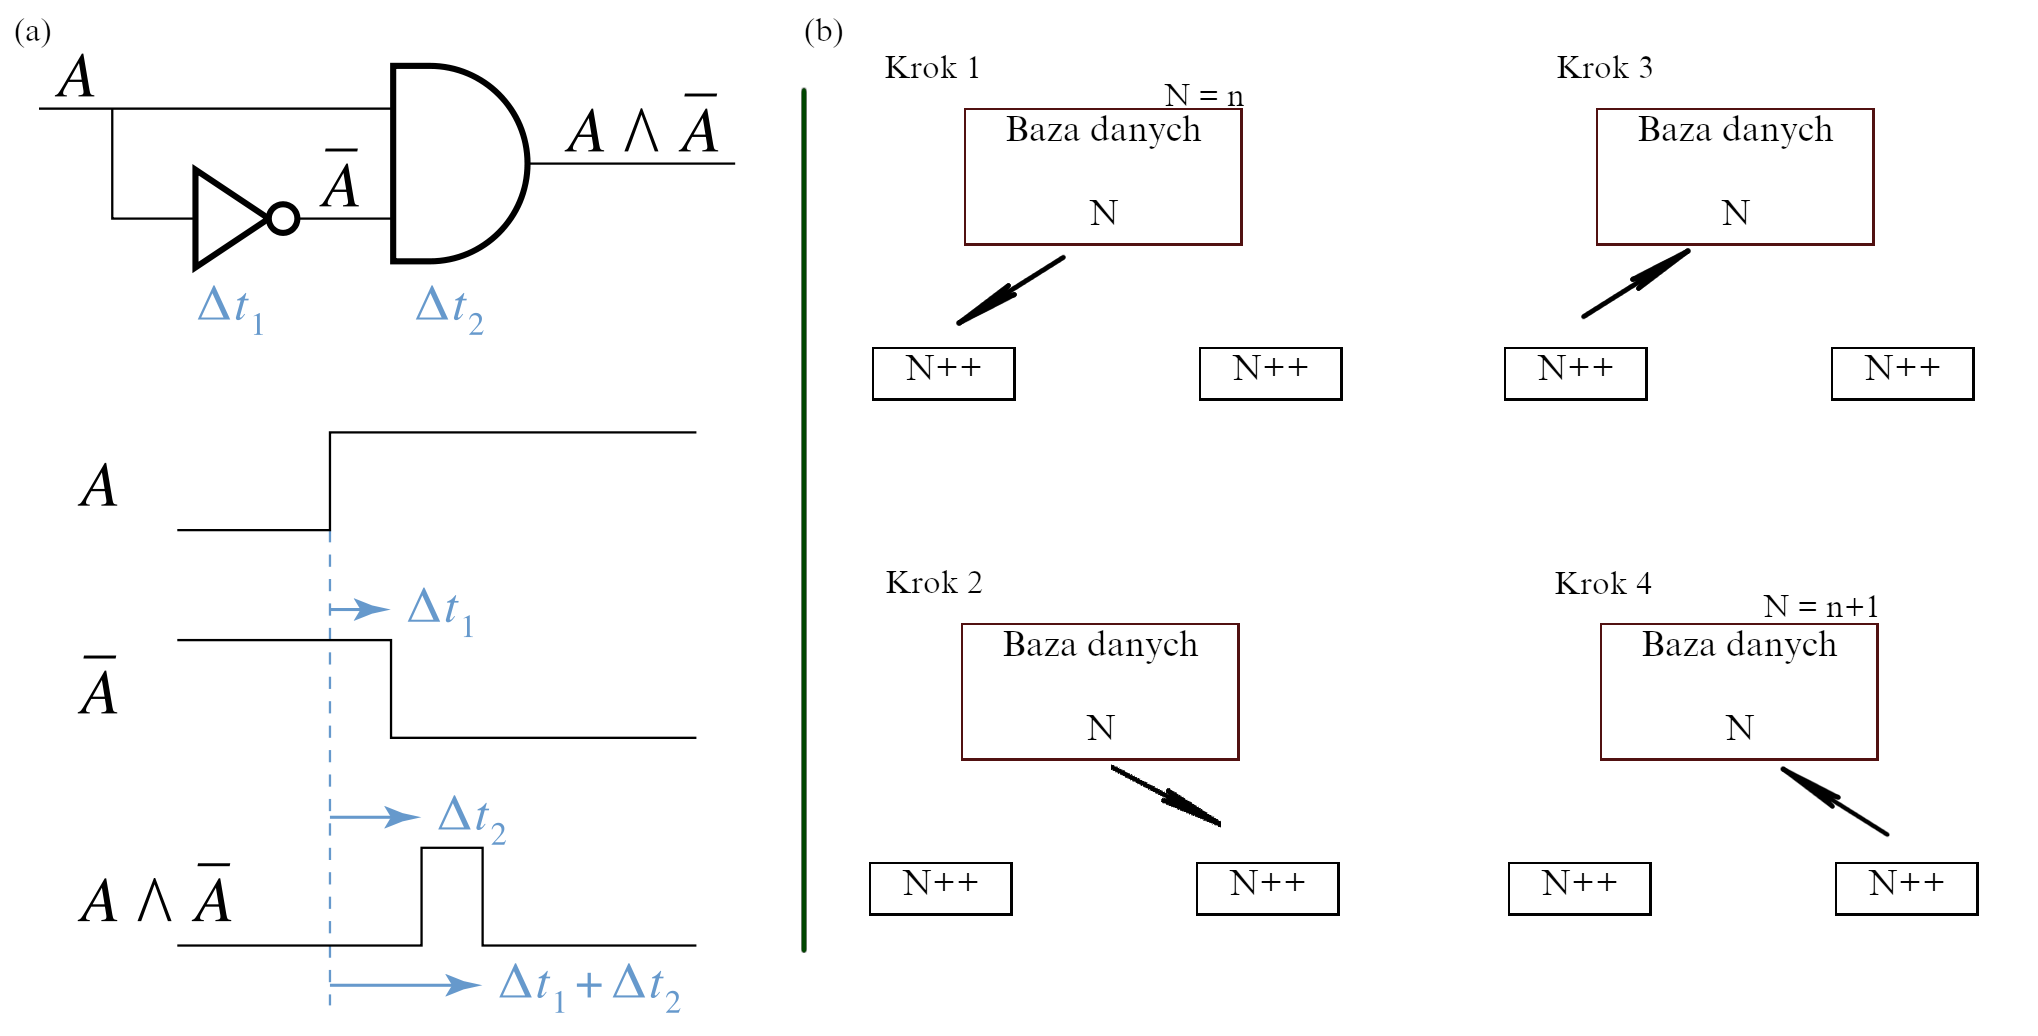
\includegraphics[width = \textwidth]{race_condition.png}
        \caption{Schematy układów w których występuje \textit{race condition}. Po lewej \textit{(a)} przykład układu elektronicznego a po prawej \textit{{b}} schemat działania programu wielowątkowego. }
        \label{race condition}
\end{figure}

W elektronice race condition to hazard spowodowany przez czas propagacji elementów układu powodujący niezamierzane efekty. Przykład układu elektronicznego w którym występuje takowy hazard jest wizualizowany na rysunku \ref{race condition}(a). 
Race condition dzieli się na statyczny i dynamiczny. Statyczny to taki w którym obserwujemy zmianę na wyjściu w chwili gdy dla układów o zerowej propagacji elementów spodziewalibyśmy się niezmienionego stanu.
W hazardzie dynamicznym spotykamy się z odwrotną sytuacją. 

W przypadku programowania wielowątkowego tego typu hazard nie jest powodowany przez czas propagacji elementów lecz przez nieznany czas i kolejność wykonywania operacji przez równolegle pracujące wątki. Przykład schematu programu dla takiego przypadku znajduje się na rysunku \ref{race condition}(b). Schemat przedstawia prostą bazę danych i dwa wątki mające za zadanie podniesienie wartości zmiennej \textit{N} o jeden.
Prosty proces zmiany zmiennej składa się z trzech oddzielnych części, pobranie wartości zmiennej, zwiększenie wartości oraz ponowne zapisanie zmiennej w pamięci. 
Dla podanego przykładu w typowym przebiegu gdy obydwa wątki zwiększą wartość zmiennej o 1 spodziewany jest wynik $N = n+2$. Jednak rzadkim przypadku może zaistnieć sytuacja że drugi wątek pobierze wartość N do obliczeń przed zapisaniem wyniku z pierwszej operacji. Spowoduje to trudny do odnalezienia i odtworzenia błąd sprawiający że zignorowane zostają obliczenia wątku który pierwszy pobrał wartość, zatem końcowy wynik będzie równy $N = n+1$.
Jest to jeden z powodów dlaczego zabezpiecza się zasoby za pomocą muteksów lub semaforów. 

Mimo sposobów na unikanie takich sytuacji programowanie wielowątkowe wymaga dużej staranności a potencjalne błędy mogą pozostawać ukryte nawet latami. To też jest powód dla którego nie należy stosować takich rozwiązań jeżeli mogą zostać pominięte\cite{multi thread problem}.
\paragraph{Zakleszczenie}

Zakleszczenie (ang. deadlock) to sytuacja gdy dwie operacje czekają na siebie wzajemnie więc żadna z nich nie może się zakończyć. 
Zakleszczenie może występować w procesach, wątkach jak i również w świecie fizycznym przykładowo w ruchu drogowym podczas blokady ronda w korku drogowym.  
Prostym przykładem takiej sytuacji jest chwila gdy dwa procesy w celu przeprowadzenia obliczeń potrzebują dwóch muteksów i w chwili gdy każdy z nich zablokuje jeden z nich przechodzą w stan wstrzymania oczekując na zwolnienie tego trzymanego przez konkurujący proces. 

 Kiedykolwiek występuje graf cykliczny zapotrzebowania zasobów deadlock może zaistnieć. 
 Powoduje to że jest to trudna sytuacja do przewidzenia w bardziej rozbudowanych programach.

W celu uniknięcia takiej sytuacji można wprowadzić pewne środki zapobiegawcze\\cite{coffman}:
\begin{itemize}
        \item Proces/wątek blokuje zasoby dopiero kiedy wszystkie są dostępne. Jest to mało optymalne rozwiązanie i może spowodować że operacja nigdy nie zostanie przeprowadzona
        \item Ustalenie mechanizmu wywłaszczania zasobów oraz hierarchii dostępu. 
        \item Przed przejściem w stan oczekiwania proces może zwolnić wszystkie przetrzymywane zasoby. 
        \item Usunięcie wymagania wyłączności. Jeżeli zasób może być używany przez wiele wątków/procesów jednocześnie to nie należy go blokować.  
        \item Projektowanie programu tak by proces/wątek wymagał jednocześnie dostępu jedynie do jednego zasobu na raz. 
\end{itemize} 

Jest to kolejny powód dla którego należy bardzo rozsądnie podchodzić do projektowania programu przy decyzji programowania wielowątkowego oraz nie nadużywać tego podejścia w sytuacjach gdy jest to niekonieczne. 

\subsubsection{Otwarte formaty danych}

Pliki o otwartych formatach danych to takie pliki tekstowe których metadane oraz semantyka jest ogólnie dostępna. 
Celem tych plików jest łatwość interpretacji zarówno przez człowieka jak i maszynę. 
Oznacza to że nie tylko są to formaty które są często implementowane w wielu programach, ale również umożliwiają ręczną manipulację danymi przez użytkownika.  
Poniżej znajdują się krótkie opisy najpopularniejszych formatów.

\paragraph{CSV}
CSV (eng. comma seperated values, wartości dzielone przecinkami) jest to prosty format plików w którym zgodnie z nazwą każda z wartości jest oddzielana przecinkiem od kolejnej. Wartości dzielą się na rekordy oddzielane znakami końca linii CRLF oraz wartości oddzielane przecinkami. Zamiast przecinków mogą być używane znaki specjalne jak średniki lub tabulatury chociaż jest to niezalecane. Jeżeli plik z danymi zawiera tablicę to ilość wartości powinna być jednakowa w każdym z rekordów. 

\paragraph{XML}

XML (eng. Extensible Markup Language) jest to uniwersalny język znaków służący do przenoszenia danych. Jego skupieniem była łatwość w pisaniu programów interpretujących ten standard.
Jest to język na podstawie którego stworzono wiele ważnych pochodnych formatów takich jak Microsoft Office XML formats, Trusted Data Format i HTML5.

Poniżej znajduje się prosty przykład takiego dokumentu:
\begin{kod}
        \lstinputlisting[language=XML]{code_source/XML.xml}
        \caption{Schematyczny przykład zawartości pliku napisanego w języku XML}
        \label{XML code}
\end{kod}

Dokument XML składa się z elementów, atrybutów oraz tagów. 
Tagi znajdują się między symbolami < > oraz każdy z nich wymaga zamknięcia przez tag o tej samej nazwie rozpoczynając się od znaku \textbackslash.
Atrybuty to pary wartość klucz znajdujące się między symbolami < > gdzie wartość zawsze musi być zawarta między znakami ".
Wartości to tekst lub kolejne elementy znajdujące się między tagami. 
Pierwsza linia to opcjonalny prolog zawierający informację o wersji XML oraz typie kodowania.  
Dokument XML musi zawierać element początkowy, w przykładowym kodzie \ref{XML code} jest to tag <root>.



\paragraph{JSON -  Java script object notation}

Mimo że nie jest standardem otwartych plików danych, lecz formą języka JavaScript to spełnia warunki czytelności przez człowieka jak i maszynę. 
Forma obiektu w tym języku stała się w przeciągu lat popularnym sposobem na przekazywanie danych między aplikacjami. Stało się tak ze względu na prostotę semantyki oraz uniwersalność. 

Każdy obiekt JSON zaczyna się symbolem \{ i kończy \} każda z wartości składa się z pary atrybut wartość przedzielona dwukropkiem, a każda z kolejnych par oddziela się przecinkiem. Typami wartości są:
\begin{itemize}
        \item liczba, 
        \item tekstowy typ danych (eng. string),
        \item logiczny typ danych,
        \item tablica - zaczyna się od [ kończy na ],
        \item obiekt,
        \item wartość pusta - null. 
\end{itemize}

Format ten wspierany jest przez wiele języków między innymi C, C++, C\#, Java, JavaScript, Perl, Python\cite{json}.

\subsubsection{Rejestr przesuwający}
Rejestr to taki układ elektroniczny którego celem jest przechowywanie oraz umożliwienie dostępu do danych. Funkcja ta jest podobna do funkcji pamięci jednak w przeciwieństwie do pamięci rejestry mogą mieć dodatkową funkcję sprzętową.
Przykładowo rejestry mogą służyć w celu komunikacji między kodem a urządzeniami wejścia/wyjścia.

Specjalnym przykładem rejestru jest rejestr przesuwający którego dane, przy sygnale z wspólnego sygnału, będą przekazywane do kolejnego miejsca przetrzymywania informacji. 
Najczęściej rejestry przesuwne są skonstruowane jako kaskada przerzutników gdzie wejście danych jest połączone z wyjściem poprzedniego.

Istnieją 4 typy rejestrów przesuwających różniących się ze względu na sposób wprowadzania i odbioru danych:
\begin{itemize}
        \item szeregowo-szeregowy,
        \item równolegle-szeregowy,
        \item szeregowo-równoległy,
        \item równolegle-równoległy zwany rejestrem buforowym  
\end{itemize} 

\newpage
\section{Projekt}

Zgodnie z dokumentacją RXHDR\_V2 \cite{master} na szesnastu wyjściach cyfrowych uzyskiwany jest sygnał o logice 0 do 1.8V o czasie trwania między 50ns a 200ns i częstotliwości osiągającej nawet do 2.5 MHz.
Sygnał ten na potrzeby rozwiązań softwarowych jest modyfikowany przez translator poziomów do poziomów logicznych 0 - 3.6V i zostaje wybierana ósemka z szesnastu kanałów przez dyskryminator.   
Tak wybrane ósemki mają nazwę 1A0-7 dla pierwszej oraz 2A0-7 dla drugiej części wyjść.   
Otrzymane sygnały należy zliczyć na płytce Arduino Due w ściśle określonym czasie oraz przekazać dane do dalszej obróbki bądź wizualizacji na zewnętrznym komputerze.

Cały proces kompilacji kodu C++ do kodu Asemblera został wykonany na kompilatorze ARM gcc 4.6.4 (linux). 

W poniższych rozdziałach opisane są proponowane sposoby wykonania tego zadania. 

\subsection{Rozwiązanie softwarowe na platformie Arduino}
\label{dzial arduino}
Założeniem rozwiązania jest bezpośrednie zliczenie sygnałów z wykorzystaniem przerwań sprzętowych w frameworku Arduino. W tym celu stosowane są wyjścia cyfrowe płytki Arduino due oraz dyskriminatora sygnałów zmniejszającego liczbę wyjść płytki z 16 do 8.
Zbocze każdego z tak dyskryminowanego sygnału  powoduje wywołanie krótkiej dedykowanej funkcji zwiększającej wartość licznika o jeden. 

Fragment kodu \ref{code_ard_IRS} jest częścią programu użytego do badań. Na potrzeby badania zostaje uwzględniony tylko pojedynczy kanał.

\begin{kod}
        \lstinputlisting[language=C++, firstline=95, lastline=117]{code_source/arduino/monocanal_rst.cpp}
        \caption{Fragment kodu użytego do testowania rozwiązania z przerwaniami systemowymi.}
        \label{code_ard_IRS}
\end{kod}


Używana płytka rozwojowa Arduino Due, używa mikrokontrolera AT91SAM3X8E w architekturze 32 bitowej o taktowaniu głównego procesora równemu 84 MHz.

Pomimo krótkiej operacji wewnątrz IRS (eng. interupt service rutine) - \textit{add} (tabela \ref{decompile add}) proces wejścia do rutyny przerwania i wyjścia zabiera nieporównywalnie więcej cykli procesora, co powoduje że cały proces wywołania przerwania jest kosztowny w czasie. 
Ilość cykli procesora koniecznych do wywołania funkcji przerwania używając nieoptymalizowanego kodu Arduino może wymagać nawet do 355 cykli procesora \cite{ard_opt_git}, dodatkowo powrót do głównego wątku programu może wymagać kolejnych 128 cykli \cite{ard_opt_git}.

\begin{table}{h}
        \begin{center}
        \caption{Estymacja ilości cyklów procesora koniecznych do wykonania instrukcji umieszczonych w funkcji \textit{add} }
        \label{decompile add}
        \begin{tabular}{c|c|c}
                kod C++ & pseudo kod Asemblera & Ilość cykli procesora \cite{cycles} \\ \hline
                val++ & LDR & 1-2 \\
                        & ADD & 1 \\
                        & STR & 1-2 \\ 
                        \hline \hline
                        &   &  3-5 
        \end{tabular}
        \end{center}
\end{table}

Pojedynczy cykl procesora zgodnie z wzorem \ref{Cykli w sec} dla układu Arduino Due trwa ~$ 11.9 ns $. 
Oznacza to że wykonanie instrukcji \textit{val ++} zgodnie z najgorszą estymacja (tabela \ref{decompile add}) trwa ~ $59.52 ns$. 
Jednak po dodaniu czasu koniecznego na wywołanie i powrót z IRS otrzymywany jest czas $ (355 + 128 + 5) * 11.9 ns =  5.8072 \mu s $. 

Podczas wywołania przerwania o tym samym priorytecie co priorytet tego właśnie wykonywanego, sygnał wywołujący zostanie zapamiętany i ewaluowany zaraz po wyjściu z właśnie wykonywanego IRS  \cite{datasheet}. 
Oznacza to że w przypadku generowania sygnałów o większej częstotliwości niż jest możliwa ich ewaluacja, doprowadzamy do sytuacji kiedy nigdy nie wrócimy do normalnego przebiegu programu. 

Zgodnie z wymaganiami projektu uzyskiwane sygnały wymagające zliczenia mogą przychodzić z częstotliwością nawet do $2.5MHz$ co oznacza kolejny sygnał przychodzący co $0.4\mu s$.
Takie wymagania oznaczają że już dla pojedynczego kanału takie rozwiązanie jest niewystarczające. 

\subsection{Rozwiązanie softwarowe w standardzie CMSIS}
Główną filozofią platformy Arduiono jest możliwość przenoszenia kodu między różnymi urządzeniami należącymi do dużej rodziny Arduino oraz łatwość programowania.
W celu osiągnięcia tych dwóch celów często poświęcana jest szybkość działania. 

Dodatkowo platforma Arduino implementuje funkcję których działanie może wpływać na pracę mikrokontrolera nawet bez ich wywoływania. 
Przykładowo na potrzeby działania funkcji \textit{milis()} konieczna jest specyficzna konfiguracja głównego zegara i cykliczne wywoływanie przerwań w celu implementacji licznika. Powoduje to kolejne spowolnienia działania programów. 


CMSIS to biblioteka udostępniająca warstwę abstrakcji dla mikrokontrolerów używających procesorów grupy ARM Cortex. 
Pozwala ona na niskopoziomowe programowanie procesorów tego typu ze skupieniem na szybkości działania.

Zgodnie z notą producenta \cite{interupt latency} w najbardziej optymalnej sytuacji dla procesora \textit{Cortex-M3} wejście do funkcji przerwania sprzętowego wymaga 12 cykli, a wyjście można osiągnąć w 10 cyklach. 
Przy tak optymistycznej estymacji możliwe byłoby osiągnięcie częstotliwości zliczeń nawet do $\frac{1}{11.9ns*27} = ~ 3.11 MHz$, jednak ponieważ zliczenia z różnych kanałów nie mogą być ewaluowane równolegle wynik ten nadal jest niewystarczający. 

Dodatkowo bez dostępu do debugera rozwiązywanie problemów pojawiających się podczas programowania w tym podejściu okazały się niewarte włożonej pracy. 

Z tych dwóch powodów rozwiązanie to zostało porzucone i nie wykonano badań w takim układzie. 

\subsection{Rozwiązanie z użyciem dodatkowego układu elektronicznego.}

Wykorzystanie rozwiązania z dodatkowym układem elektroniki przy wykorzystaniu frameworku Arduino. Celem dodatkowego elementu elektronicznego jest ułatwienie odczytu zliczeń przez mikrokontroler oraz zmniejszenie wymaganej częstotliwości zliczeń. 

\subsubsection{Układ liczników zewnętrznych}
\label{section licziki}

W celu rozwiązania problemu wysokiej częstotliwości zliczeń otrzymywanych z układu RXHDR\_V2 \cite{master} zastosowano zestaw ośmiu binarnych liczników 4-bitowych \cite{licznik doc}. 


\begin{figure}[]
        \centering
        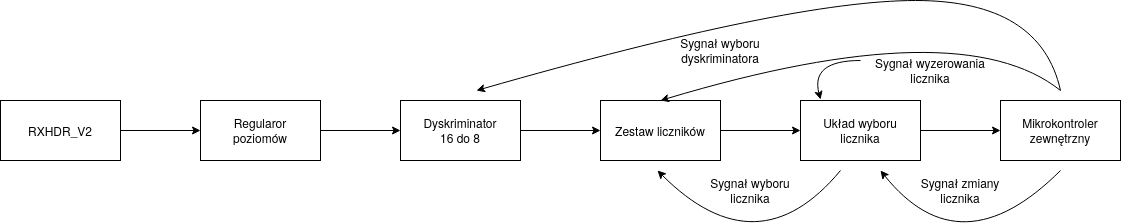
\includegraphics[width=\textwidth]{Elektronika_flow_chart.png}
        \caption{Schemat działania układu liczników zewnętrznych i sygnałów kontrolujących}
        \label{licznik flowchart}
\end{figure}

Schemat ideowy układu znajduje się na obrazku \ref{licznik flowchart}.
Na tym schemacie znajdują się sygnały kontrolujące pracę układu. Poniżej zdefiniowane jest nazewnictwo sygnałów na schematach elektronicznych i ich funkcja.  
\begin{itemize}
        \item ReadCLC - Sygnał zmiany licznika - pojedynczej przejście stanu z niskiego na wyskoki powoduje wybór kolejnego licznika do odczytu
        \item RC\_B - Sygnał wyzerowania licznika - stan niski powoduje wyzerowanie liczników i ustawienie układów do stanu początkowego.
        \item DIS\_S - Sygnał wyboru dyskryminatora - Stan niski powoduje wybranie sygnałów 1A0-7 a wysoki 2A0-7
        \item ENP0-7 - Sygnał wyboru licznika - osiem osobnych linii których stan niski pozwala na wybór licznika do odczytu. Podczas odczytu tylko jeden z sygnałów powinien być w stanie niskim reszta powinna utrzymywać stan wysoki. 
\end{itemize}
Sygnał otrzymywany przez układ RXHDR\_V2 jest przepuszczany przez translator poziomów w celu zmiany logiki z 0-1.8$V$ do 0-3.6$V$. Następnie z 16 kanałów zostaje wybrane 8, tak opracowane sygnały trafiają na układ liczników.

\paragraph{Układ liczników \cite{licznik doc}\cite{slave}}

4-bitowy binarny licznik SN74LV161A ma 9 wejść logicznych. 
W tym układzie licznik znajduje się w następującej konfiguracji:
\begin{itemize}
        \item $CLC$ - Tu podawany jest sygnał zliczeń i on jest zliczany aż do przepełnienia licznika.
        \item $\overline{CLR}$ - Połączone z linią RC\_B, stan niski powoduje wstrzymanie pracy i wyzerowanie wartości przechowywanych w liczniku. 
        \item $ENT,ENP$ - w celu stabilizacji układu na czas odczytywania wartości chcemy wstrzymać zliczanie dlatego też ustalamy stan wysoki dla wejścia ENT i wejście ENP łączymy z kanałem ENP0-7 odpowiadającym odpowiedniemu licznikowi.
        Sprawia to że wraz z wyborem licznika układ ustala swój stan i nie zmienia go aż do chwili wyboru następnego. 
        Jest to sposób na uniknięcie niepewności i błędów wynikających z odczytywania zmieniającej się wartości, jednak powoduje to powstanie czasu martwego w układzie podczas którego wartości nie będą zliczane na odczytywanym liczniku.
        \item $A,B,C,D$ - funkcja ładowania wartości nie jest używana wejścia te są uziemione
        \item $\overline{LOAD}$ - funkcja ładowania wartości nie jest używana wejście to jest uziemione
\end{itemize} 

Na wyjściu wykorzystane są jedynie linie Q0-3 to one podają binarnie przechowywaną wartość. 
Tak skonfigurowane liczniki będą zliczać wartości otrzymywane przez wejście $CLC$ aż do osiągnięcia wartości 16 kiedy to licznik zostaje przepełniony i podawana przez niego wartość wraca do 0. 

\paragraph{Układ wyboru sygnału}

Celem tego układu jest zmiana sygnału zmiany licznika na sygnał wyboru licznika. W tym celu wykorzystany jest rejestr przesuwany. 
Wybrany układ służący temu zadaniu to SN74LV164A\cite{shift doc}, jest on szeregowo-równoległym rejestrem co oznacza ze dane wejściowe są dostarczane szeregowo a otrzymywana jest informacja równoległa która jest przesuwana wraz z kolejnymi sygnałami zegara. Dokumentacja rejestru SN74LV164A mówi o dwóch wejściach jednak są one bezpośrednio wyprowadzane na bramkę logiczną AND co sprawia że układ ten spełnia warunek pojedynczego wejścia rejestru szeregowo-równoległego. W konfiguracji tego układu gdzie oba wejścia są ze sobą zwarte, bramka logiczna AND jest ignorowana.
Schemat układu wyboru licznika znajduje się rysunku \ref{wybor schema}. 

\begin{figure}
        \begin{multicols}{2}
                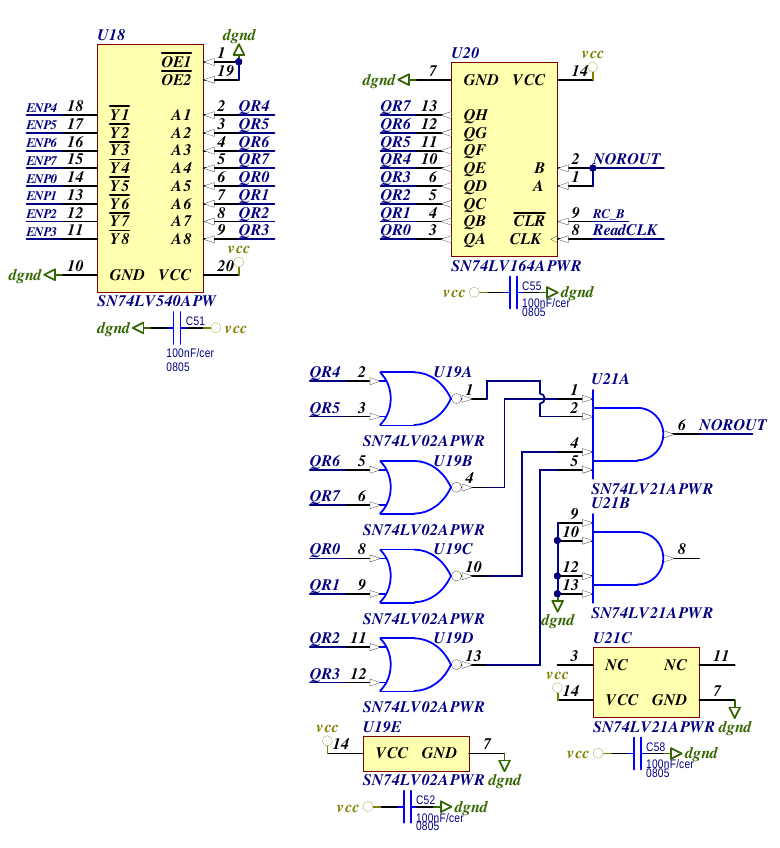
\includegraphics[width=0.45\textwidth]{shift_register.png}
                \caption{Schemat układu wyboru licznika wykorzystujący rejestr przesuwny.}
                \label{wybor schema}
                \par
                \hfill
                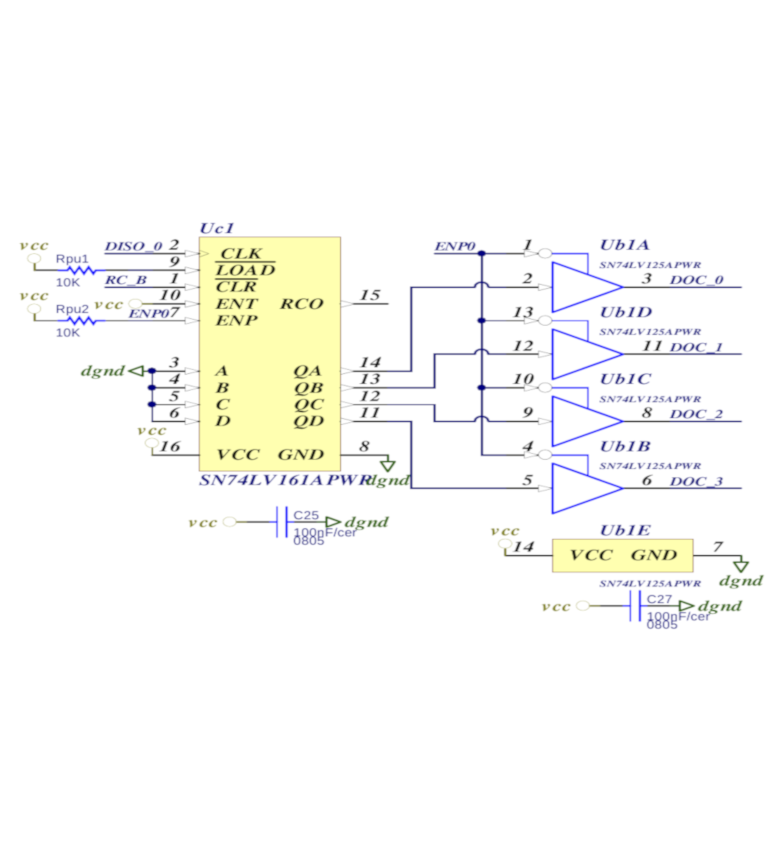
\includegraphics[width=0.45\textwidth]{Licznik.png}
                \caption{Schemat konfiguracji jednego z używanych liczników wraz z częścią multipleksera wyjściowego.}
                \label{licznik}
                \par
                \hfill
        \end{multicols} 
\end{figure}

W celu osiągnięcia efektu pojedynczej wartości logicznej która przesuwa się z każdym rosnącym zboczem sygnału na wejściu rejestru musimy dostarczyć pojedynczy niski, stan podczas pierwszego cyklu pracy, a następnie trzymać stan wysoki aż do chwili potrzeby powtórzenia cyklu. 
Za pomocą bramek NOR układu SN74LV02A oraz bramek AND układu SN74LV21A osiągamy równanie logiczne:
\begin{equation}
        NOROUT = \overline{(QR1*QR2)} + \overline{(QR3*QR4)} + \overline{(QR5*QR6)} + \overline{(QR7*QR8)}
\end{equation}
Gdzie:
\begin{itemize}
        \item $NOROUT$ - Sygnał wejściowy rejestru 
        \item $QR1-8$ - Wyjścia rejestru. 
\end{itemize}

\begin{table}
        \centering
        \caption{Cykl działania rejestru przesuwnego układu wyboru licznika}
        \label{shift sygnal}
        \begin{tabular}{lccccccccc}
                Czas &$QR1$&$QR2$&$QR3$&$QR4$&$QR5$&$QR6$&$QR7$&$QR8$  &NOROUT\\ \hline     
                T1&H&H&H&H&H&H&H&H &L\\
                T2&L&H&H&H&H&H&H&H &H\\
                T3&H&L&H&H&H&H&H&H &H\\
                T4&H&H&L&H&H&H&H&H &H\\
                T5&H&H&H&L&H&H&H&H &H\\
                T6&H&H&H&H&L&H&H&H &H\\
                T7&H&H&H&H&H&L&H&H &H\\
                T8&H&H&H&H&H&H&L&H &H\\
                T9&H&H&H&H&H&H&H&L &H\\
                T10&H&H&H&H&H&H&H&H &L\\
        \end{tabular}
\end{table}

Sekwencja sygnału pokazana jest w tabeli \ref{shift sygnal}. Na tej wizualizacji widać że gdyby w konfiguracji zastąpić linię $QR8$ połączeniem do zasilania możliwe byłoby ograniczenie liczby sekwencji w cyklu do 8. Jednak dzięki tej pojedynczej sekwencji gdy żaden z liczników nie jest odczytywany otrzymujemy cykl podczas którego żaden z liczników nie jest zablokowany i wszystkie kontynuują liczenie. 

W ten sposób otrzymywany sygnał następnie jest negowany przez układ SN74LV540 i dostarczany do multipleksera pokazanego na rysunku \ref{licznik}.
Tu zestaw wzmacniaczy operacyjnych sprawia ze tylko tylko licznik dla odpowiadającego sygnału ENP o niskim stanie ustala stan na zewnętrznych wyjściach. 

\paragraph{Czas martwy i szybkość odczytu układu licznika}
Podczas odczytu licznika informacja o zliczeniach zostaje tracona oznacza to że układ ten generuje czas martwy. 
Procentowa długość tego czasu może być wyznaczona na podstawie wzoru:
\begin{equation}
        T_d = \frac{T_o/N_l}{T_o+T_e} * 100\%
\end{equation}
Gdzie:
\begin{itemize}
        \item $T_d$ - procentowy czas martwy licznika.
        \item $T_o$ - czas odczytu.
        \item $N_l$ - liczba liczników w sekwencji odczytu. W używanej konfiguracji jest to osiem liczników. 
        \item $T_e$ - czas pustego cyklu.
\end{itemize}

Oznacza to że przedłużając czas pustego cyklu zmniejszamy czas martwy układu, jednak ponieważ liczniki mogą jedynie 16 stanów to konieczne jest odczytanie ich przed zliczeniem 16 liczby. 
Oznacza to że:
\begin{equation}
        T_o+T_e * F \leqslant 15
\end{equation}
        Gdzie:
\begin{itemize}
        \item $F$ - spodziewana częstotliwość zliczeń
\end{itemize}

Dla podanych wymagań: 2.5 miliona zliczeń na sekundę, można wyliczyć że suma czasu odczytu i pustych sekwencji powinna być mniejsza niż 6$\mu s$.
Oznacza to że sekwencja odczytu powinna zmieścić się w 504 cyklach procesora. 

\subsubsection{Oprogramowanie mikrokontrolera}

Zadaniem mikrokontrolera jest odebranie danych z układu wspomagającego w czasie uniemożliwiającym przepełnienie liczników i wysłanie sformatowanych danych na komputer zewnętrzy. 

\paragraph{Wymagane połączenie}
W celu utworzenia funkcjonującego układu akwizycji zliczeń konieczne jest połączenie kablem USB2.0 typ A/micro-USB typ B między komputerem sterującym a natywnym portem Arduino Due (Port bliżej przycisku resetu).

Dodatkowo wymagane jest połączenie z płytką zewnętrzną. Konieczne połączenia to:
\begin{itemize}
        \item Połączenia $DOC\_0-4\_ext$ w domyślnej konfiguracji powinny być połączone z wyjściami arduino o pinach 33-36 - są to wyjścia liczników.
        \item $RC\_B\_ext$ - arduino pin 46 - wyjście sygnału resetu liczników 
        \item $DIS\_S\_ext$ - arduino pin 46 - wyjście sygnału wyboru dyskryminatora
\end{itemize}

Są to wyjścia w domyślnej konfiguracji i można dokonać zmiany poprzez modyfikację pliku \textit{USER\_CONFIG.h}.



\paragraph{Akwizycja danych}
Dane otrzymywane z zewnętrznego układu elektronicznego (dział \ref{section licziki}) mają postać binarnej liczby 4-pozycyjnej rosnącej do wartości 15 a następnie zawijające się ponownie do liczby 0. 
Dzięki tej formie prezentacji danych po odczytaniu stanów logicznych na urządzeniu peryferyjnym i odpowiednim przesunięciu logicznym w prosty sposób otrzymujemy wartość na liczniku. 
Podejście to jednak wymaga specyficznego połączenia oraz uwzględnienia potencjalnego przepełnienia licznika. 

W jednym cyklu akwizycji zostaje wybierany pierwsze osiem liczników 1A0-7 następnie przez czas akwizycji, korygowanej o czas martwy, zbierane są dane z liczników i dodawane do miejsca w tablicy odpowiadającemu odpowiedniemu licznikowi, następnie zmieniana jest ósemka badanych liczników i proces ponownie jest powtarzany. 

Proces akwizycji danych musi być bardzo dokładnie kontrolowany pod względem czasu wykonania.
Czas pobierania danych jest regulowany przez ilość pętli Podczas których dokonywana jest akwizycja danych. 
Przykład tej pętli znajduje się w fragmencie kodu \ref{code aqw}.

\begin{kod}
        \lstinputlisting[language=C++, firstline=76, lastline=103]{code_source/arduino/final.cpp}
        \caption{Fragment kodu odpowiedzialnego za akwizycję danych}
        \label{code aqw}
\end{kod}

Jak widać ilość iteracji jest ustalana przez wymagany czas w milisekundach po korekcjach o czas martwy licznika oraz z uwzględnieniem ilości czasu przypadającego na pojedynczą pętlę. 
Warunkiem koniecznym takiego podejścia jest stały czas wykonywania iteracji pętli. 
Różnice w czasie mogą być powodowane przez operacje dostępu do pamięci kiedy to w różnych iteracjach stosujemy dostęp do pamięci a w innych wykorzystujemy wcześniej przygotowane rejestry.
Drugim powodem mogą być rozwidlenia pracy programu, sytuacje kiedy przebieg programu jest uwarunkowany wynikiem jakiegoś warunku i dwie drogi potrzebują różną ilość cykli procesora na wykonanie. 
W celu analizy takich sytuacji przydatna jest analiza skompilowanego kodu c do kodu asemblera.
Fragment krytycznej części programu jest przedstawiony w wycinku kodu \ref{asembly}.

\begin{kod}
        \lstinputlisting[language={[Motorola68k]Assembler},firstline=30, lastline=48]{code_source/asembler/loop_final.S}
        \caption{Fragment kodu asemblera utworzonego przez kompilację części kodu \ref{code aqw}. }
        \label{asembly}
\end{kod}

Po analizie kodu \ref{asembly} można stwierdzić że nie zdarza się sytuacja żeby w różnych iteracjach występowała różna ilość dostępów do pamięci.
Jak jednak widać w fragmencie programu \ref{code aqw} w przypadku wystąpienia przepełnienia licznika konieczne jest dodanie wartości pełnego licznika do otrzymanej liczby. 
Powoduje to że wymagana jest dodatkowa instrukcja add.

Jednak proces warunkowego dodania jest realizowany przez specyficzną instrukcję it.
Należy ona do zestawu instrukcji Thumb®-2 i pozwala na uniknięcie problemów wynikających z warunkowej zmiany biegu programu dla krótkich instrukcji. 
Zgodnie z dokumentacją\cite{cycles} cortex-M3 czas potrzebny na wykonanie tej instrukcji to jeden cykl procesora, jednak jest sprecyzowane że instrukcja może być dołączona do następnej instrukcji pozwalając na wykonanie w tym samym czasie co następna komenda.
Tak się dzieje w przypadku spełnienia warunku gt (eng. greater then - większy niż) poprzedniej instrukcji cmp. Jednak jeżeli warunek ten nie zostaje spełniony to ewaluacja instrukcji it zwiększa się do jednego cyklu i przechodzi do warunku else (druga instrukcja w kolejności).
Cały ten proces sprawia że tak samo w przypadku spełniania warunku gt jak i w przypadku niezgodności ten fragment kodu wymaga dwóch cykli procesora.
$$it(1c) + rsb(1c) = it(0c) + add(1c) + rsb(1c)$$

\paragraph{Komunikacja z komputerem zewnętrznym}
Ze względu na fakt że proces akwizycji danych jest tak wrażliwy na wszelkie zmiany ilości poleceń konieczne jest wyłączenie obsługi przerwań w trakcie wykonywania kluczowego fragment programu. 
Sprawia to że w trakcie akwizycji obsługa komunikacji z zewnętrznymi urządzeniami przez układy komunikacji seryjnej jest niemożliwa. 
Oznacza to że wymagana jest bardzo dokładna obsługa komunikacji z zwróceniem szczególnej uwagi na potencjalne błędy. 

W tabeli \ref{komunikacja} znajdują się komendy i odpowiedzi stosowane w komunikacji między urządzeniami. 
Forma wszelkich stałych komunikacyjnych znajduje się w osobnym pliku \textit{USER\_CONFIG.h} pozwalającym na łatwą zmianę prezentowanych komend.

\begin{table}
        \centering
        \caption{Tabela komend stosowanych w celu komunikacji między komputerem zewnętrznym a mikrokontrolerem}
        \label{komunikacja}
        \begin{tabularx}{\textwidth}{|c|c|X|}
                \hline
                komenda & odpowiedź & opis \\ \hline

                \textbackslash n & Ready to read\textbackslash n & 
                Krótki znak rozpoczynający komunikację.
                Po otrzymaniu tego symbolu mikrokontroler wstrzymuje proces akwizycji i oczekuje na dalsze polecenia.
                Przed wysłaniem dowolnej komendy konieczne jest poprzedzenie tym symbolem, w celu upewnienia się że mikrokontroler jest gotowy na zmianę trybu pracy.
                \\ \hline

                42a\textbackslash n & 42b\textbackslash n& Krótka komenda, nie zmieniająca nic w pracy licznika. Pozwala na sprawdzenie komunikacji między licznikiem a komputerem zewnętrznym. \\ \hline

                atm{TIME}\textbackslash n & TIME\textbackslash n& TIME to czas w milisekundach, jest on ustalany jako czas akwizycji licznika. Musi on być podany jako liczba całkowita.\\ \hline

                stp\textbackslash n& fin\textbackslash n& Wstrzymuje pracę licznika. \\ \hline

                srt\textbackslash n& - & Rozpoczyna pracę licznika \\ \hline

        \end{tabularx}
\end{table}

Po zakończonej akwizycji dane zostają wysłane w jednym kawałku na komputer zewnętrzny w postaci:
\begin{itemize}
        \item \detokenize{<~+~>}'\textbackslash n'
        \item {Nazwa kanału}'\textbackslash t'{wynik}'\textbackslash n'
        \item \detokenize{~<+>~}'\textbackslash n'
\end{itemize}
Przykład komunikacji wygląda następująco:
\begin{lstlisting}
<~+~>
1A1     1234
1A2     1234 
    ...
2A8     1234
~<+>~
\end{lstlisting}

Długi symbol początku i końca danych pozwala na łatwe odnalezienie fragmentu komunikacji które zawiera dane pomiarowe. 

\subsection{Program kontroli, wizualizacji oraz archiwizacji danych}

Program używany na komputerze podłączonym do mikrokontrolera został napisany z wykorzystaniem języka Python i frameworku PyQt5.
Szczegółowe zadania programu to:
\begin{itemize}
        \item Komunikacja z mikrokontrolerem w celu:
        \begin{itemize}
                \item Upewnienia się o sprawnym działaniu programu na płytce arduino.
                \item Ustawienia czasu akwizycji.
                \item Odebraniu danych o zliczeniach. 
        \end{itemize}
        \item Umożliwienie wyboru konfiguracji pracy programów przez interfejs użytkownika.
        \item Analiza otrzymanych danych pomiarowych.
        \item Wizualizacja danych pomiarowych.
        \item Archiwizacja danych pomiarowych w wybranym formacie danych.
\end{itemize}

Program podzielony jest na dwie zależne od siebie części. Fasadę (eng. front-end) zawierającą graficzny interfejs użytkownika (eng. GUI) oraz wnętrze (eng. back-end).

\paragraph{Wnętrze}

Głównym celem tej części programu jest komunikacja z mikrokontrolerem. 
W tym celu wykorzystywana jest biblioteka PySerial\cite{pyserial} pozwalająca na łatwą obsługę portu szeregowego USB. 

By umożliwić jednoczesną wizualizację danych wraz z odbieraniem informacji z mikrokontrolera konieczna była implementacja wątku zajmującego się ciągłym odbiorem danych. 
Dlatego też jedyny cel funkcji \textit{back\_end\_deamon} jest nasłuchiwanie w ciągłej pętli oraz zapisywanie danych w logu komunikacyjnym. 
Na podstawie klasy tego logu wątek główny programy okresowo aktualizuje klasę \textit{CountRateData} która jest wykorzystywana przez fasadę w celu wizualizacji. 

Schemat elementów programu wraz z mutexami które chronią przed błędami jednoczesnego dostępu zwizualizowane są na rysunku \ref{program zapotrzebowanie}.

\begin{figure}
        \centering
        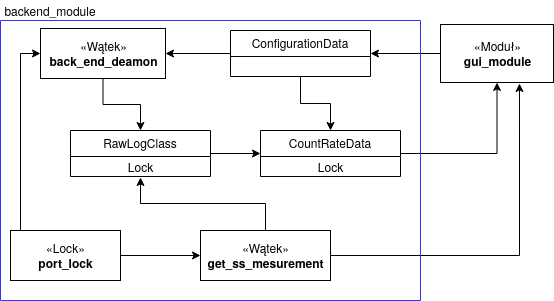
\includegraphics[width=0.65\textwidth]{Schemat_zapotrzebowania.png}
        \caption{Schemat zapotrzebowania na zasoby przez elementy programu}
        \label{program zapotrzebowanie}
\end{figure}

Klasa \textit{CountRateData} oprócz przetrzymywania danych o zliczeniach dla każdego kanału również zawiera informacje o czasie akwizycji, dzięki temu możliwe jest przekazywanie informacji do wizualizacji już jako częstotliwości zliczeń. 

Dodatkową funkcjonalnością programu jest możliwość przeprowadzenia pojedynczego badania nazywanego \textit{Single Shoot} lub skrótowo \textit{ss}.
Funkcja ta pozwala na wizualizację w postaci wykresu słupkowego pojedynczego badania w przeciwieństwie do domyślnego układu wizualizacji który jest stale aktualizowany. 
W celu przeprowadzenia takiego pomiaru wątek \textit{get\_ss\_mesurements} zamyka mutexy odpowiedzialne za port seryjny oraz Klasę logu. 
Tym sposobem wstrzymywane są inne funkcje programu aż do zakończenia pomiaru \textit{Single Shoot}.
Pomiar kończy się komendą wstrzymania pracy licznika pozwalając na zmianę konfiguracji przed kolejnymi pomiarami.  

Dane pomiarowe są zapisywane w chwili gdy: Program zostanie zamknięty, wciśnięty zostanie guzik \textit{force save}, lub minie czas auto zapisu ustawiany w interfejsie użytkownika. 

Przed zapisem tworzony zostaje folder z aktualną datą, w formacie DD-MM-YYYY, w wybranej przez użytkownika ścieżce. Nazwa pliku to godzina zapisu pliku w formacie HH:MM
Pliki są zapisywane w ustalonym formacie: JSON lub CSV.

Archiwizacja danych z akwizycji \textit{Single Shoot} jest przeprowadzana zaraz po zakończeniu pomiaru w osobnym folderze zgodnie z wcześniej przedstawioną zasadą. 

\paragraph{Fasada}
\begin{figure}
        \begin{multicols}{2}
        
        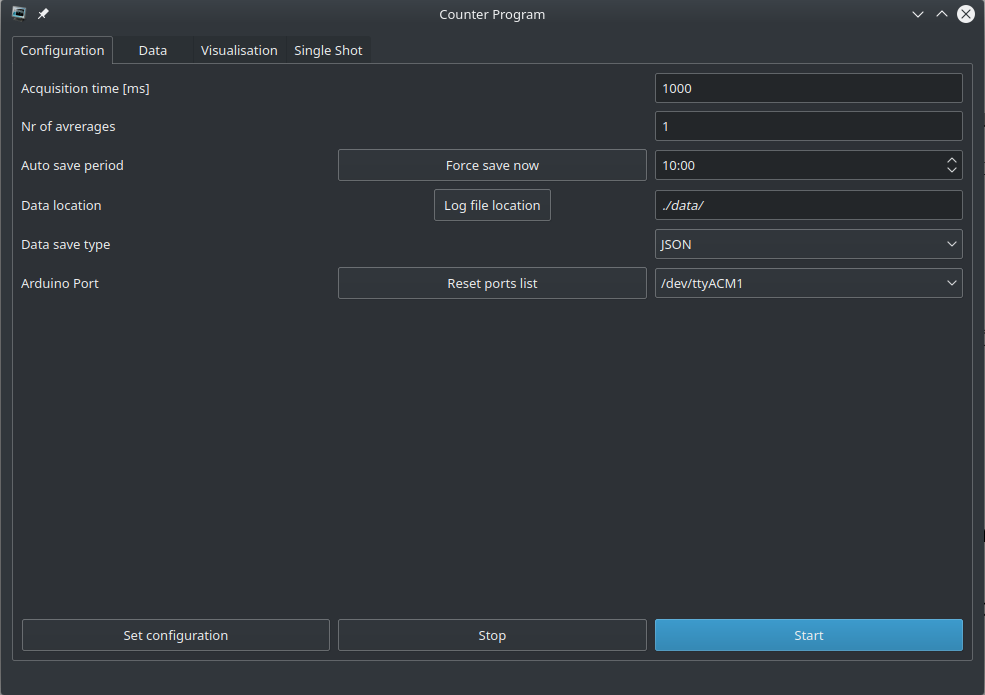
\includegraphics[width=0.49\textwidth]{configuration.png}\par
        
        
        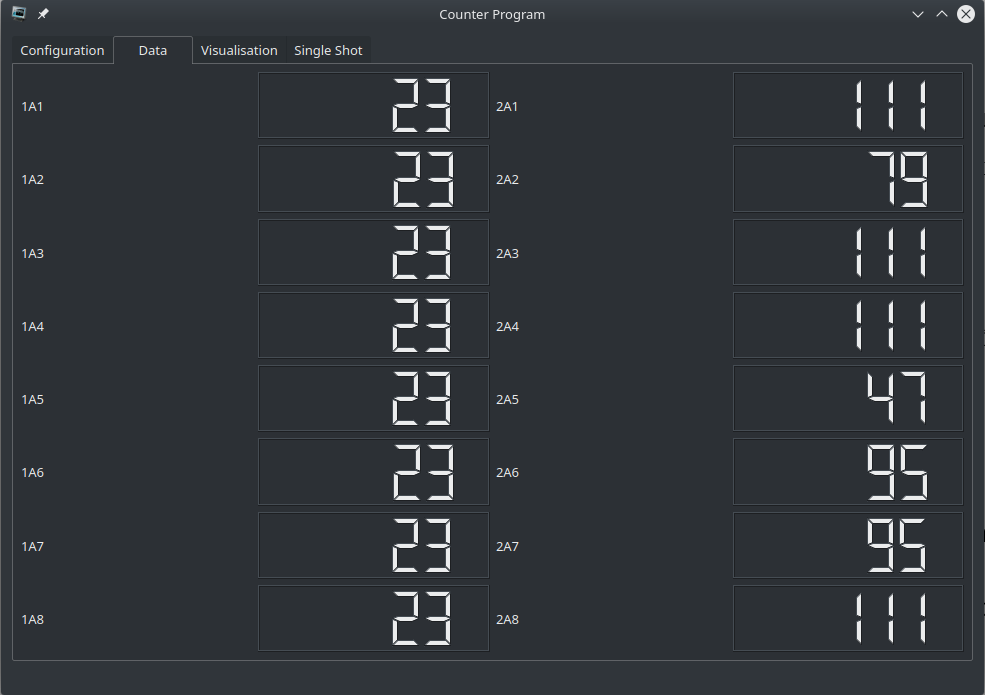
\includegraphics[width=0.49\textwidth]{digits.png}\par
        
        
        \end{multicols}\hfill
        
        \begin{multicols}{2}
        
        
        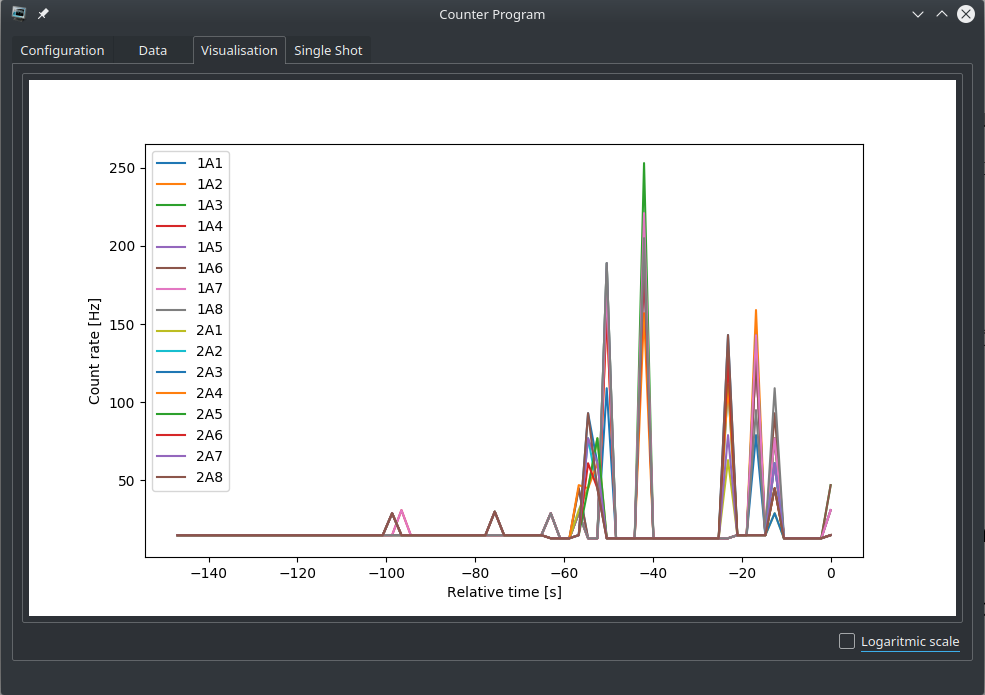
\includegraphics[width=0.49\textwidth]{wizualization.png}\par
        
        
        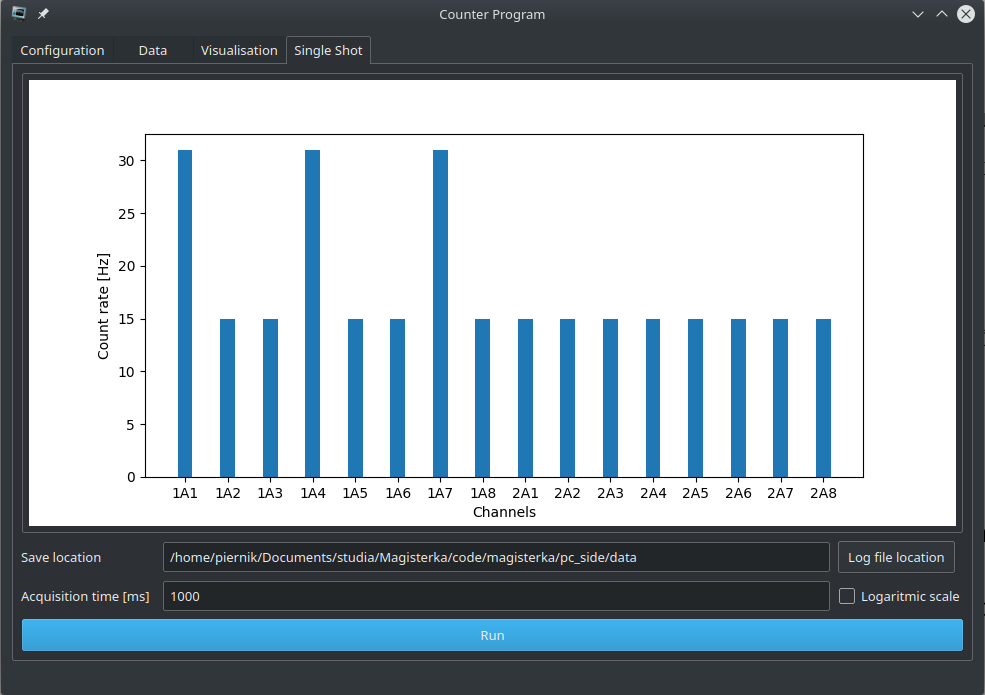
\includegraphics[width=0.49\textwidth]{wiz_ss.png}\par
        
        \end{multicols}
        \caption{Wygląd interfejsu użytkownika (linux)}
        \label{Gui pic}
        \end{figure}

Gotowy interfejs graficzny widoczny jest na rysunku \ref{Gui pic}. Jest on podzielony na cztery zakładki:
\begin{itemize}
        \item Configuration - miejsce pozwalające na rozpoczęcie pracy licznika, zatrzymanie i wszelką konfigurację dotyczącą pracy programu. 
        \item Data - prezentacja danych w postaci liczbowej 
        \item Visualization - prezentacja danych w relatywnej dziedzinie czasu. 
        \item Single Shot - Zakładka odpowiedzialna za przeprowadzenie pojedynczego badania.
\end{itemize}

Za interfejs użytkownika odpowiedzialny jest główny wątek programu, instancje klasy QTimer\cite{doc pyqt} generują one sygnały aktualizujące dane licznika oraz stgnały aktualizacji wykresu zliczeń. 
Do generowania grafik zastosowana została biblioteka matplotlib\cite{doc matplotlib}. 

Przy wykresach znajduje się pole które po odznaczeniu pozwala na wizualizację danych w logarytmicznej sali częstotliwości zliczeń.

\newpage
\section{Wyniki badań}

\subsection{Rozwiązanie softwarowe na platformie Arduino}

Przeprowadzono testy polegające na bezpośrednim zliczaniu sygnałów generowanych przez generator zewnętrzy. 
Napięciem, kształtem oraz długością odpowiadały tym produkowanym przez układ RXHDR\_V2.

Przeprowadzono po pięć badań na każdą częstotliwość i wyliczono błąd względem spodziewanego wyniku. 
Czas akwizycji ustalono na jedną sekundę sprawiając że liczba spodziewanych zliczeń jest równa częstotliwości generowanych sygnałów.

Wyniki znajdujące się w tabeli \ref{rts table} zwizualizowane są na wykresie \ref{rts wyniki}.


\begin{figure}[]
        \centering
        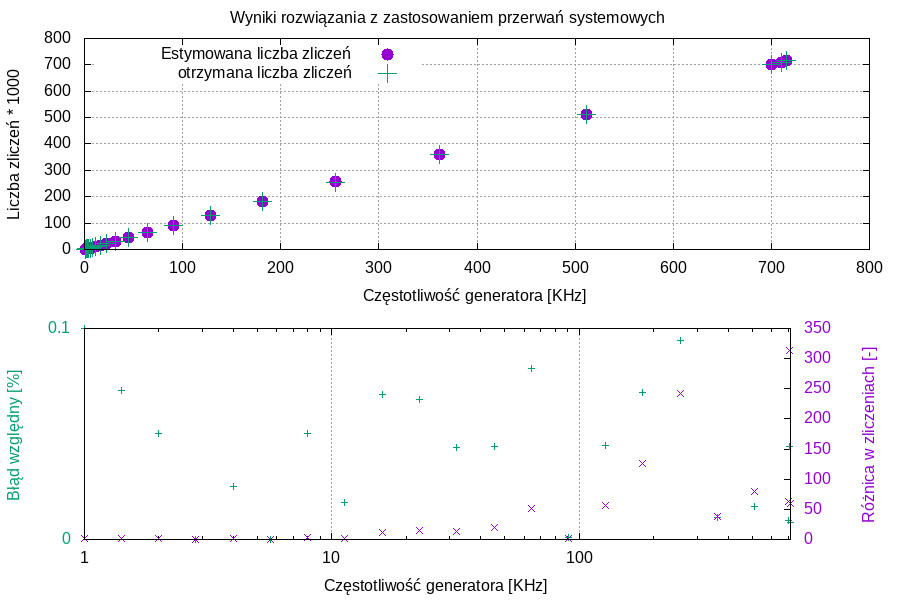
\includegraphics[width=\textwidth]{rts.jpg}
        \caption{Wyniki testów z wykorzystaniem przerwań systemowych}
        \label{rts wyniki}
\end{figure}

\begin{table}
        \centering
        \caption{Wyniki rozwiązania z zastosowaniem przerwań systemowych}
        \label{rts table}
        \begin{tabular}{|c|c|c|c|c|}  
                \hline 
                Częstotliwość [kHz] & Estymowana ilość & Otrzymana ilość & Różnica  & Błąd względny [\%]\\ 
                &  zliczeń &  zliczeń & w zliczeniach & \\ \hline
                1 & 1000 & 1001 & 1 & 0.1000\\ \hline 
                1.414 & 1414 & 1415 & 1 & 0.0707\\ \hline 
                2 & 2000 & 2001 & 1 & 0.0500\\ \hline 
                2.82 & 2820 & 2820 & 0 & 0.0000\\ \hline 
                4 & 4000 & 3999 & 1 & 0.0250\\ \hline 
                5.65 & 5650 & 5650 & 0 & 0.0000\\ \hline 
                8 & 8000 & 7996 & 4 & 0.0500\\ \hline 
                11.3 & 11300 & 11298 & 2 & 0.0177\\ \hline 
                16 & 16000 & 15989 & 11 & 0.0688\\ \hline 
                22.62 & 22620 & 22605 & 15 & 0.0663\\ \hline 
                32 & 32000 & 31986 & 14 & 0.0438\\ \hline 
                45.25 & 45250 & 45230 & 20 & 0.0442\\ \hline 
                64 & 64000 & 63948 & 52 & 0.0813\\ \hline 
                90.5 & 90500 & 90499 & 1 & 0.0011\\ \hline 
                128 & 128000 & 127943 & 57 & 0.0445\\ \hline 
                181 & 181000 & 180874 & 126 & 0.0696\\ \hline 
                256 & 256000 & 255758 & 242 & 0.0945\\ \hline 
                362 & 362000 & 361962 & 38 & 0.0105\\ \hline 
                512 & 512000 & 511920 & 80 & 0.0156\\ \hline 
                700 & 700000 & 699937 & 63 & 0.0090\\ \hline 
                710 & 710000 & 709686 & 314 & 0.0442\\ \hline 
                715 & 715000 & 714941 & 59 & 0.0083\\ \hline
        \end{tabular}
\end{table}

Wyniki pokazują dokładność mieszczącą się w  1\textperthousand, 
jednak błąd w otrzymanym wyniku zależy od częstotliwości generowanych zliczeń.
Może to być spowodowane interferencją przerwania powodującego zliczenie z innymi przerwaniami wymaganymi do działania mikrokontrolera.

Po osiągnięciu częstotliwości granicznej > 0.715 [MHz] program mikrokontrolera przestaje wysyłać dane na komputer zewnętrzny.
Jest to spowodowane tym że zaraz po wyjściu z obsługi przerwania systemowego program natychmiast zaczyna obsługę następnego przerwania. 
Liczba graniczna pozwala przybliżyć czas konieczny na wykonanie jednego przerwania na podstawie przekształcenia wzoru \ref{Cykli w sec}. 
$$ t_p = \frac{1}{f_p} = \sim 1.3986 [\mu s] $$
$$ N_c = \frac{t_p}{t_c} =  \frac{1.3986 \mu s}{11.9 ns} =\sim 118$$
gdzie: \\
        \indent $t_p$ -  czas potrzebny na obsługą przerwania\\
        \indent $t_c$ -  czas jednego cyklu procesora (dział \ref{dzial arduino} ) \\
        \indent $f_p$ -  częstotliwość graniczna przerwań \\
        \indent $N_c$ -  ilość cykli koniecznych na pojedyncze przerwanie \\

Liczba cykli na przerwanie jest mniejsza niż ta szacowana w dziale \ref{dzial arduino} (355 + 128)\cite{ard_opt_git}, wynika to z faktu że poprzednia estymacja była wykonana dla najgorszego przypadku dla nieoptymalizowanego kodu.
Mimo lepszych osiągów niż te szacowane wynik ten nadal odbiega od optymalnego czasu wywołania przerwania (12 + 10) \cite{interupt latency} i wciąż jest znacznie poniżej wymagań projektu. 

Dodatkowe testy potwierdziły że wraz z zwiększeniem ilości badanych kanałów częstotliwość graniczna zmniejsza się jak $\frac{1}{n}$ gdy $n$ to ilość badanych kanałów. 


\newpage
\section{Podsumowanie}

\newpage
\begin{thebibliography}{99}

        \bibitem{arch}
        John L. Hennessy, David A. Patterson 
        \textit{Computer Architecture: A Quantitative Approach  5th Edition }
        The Morgan Kaufmann Series in Computer Architecture and Design

        \bibitem{gcc}
        988-2019 Free Software Foundation
        \textit{Using GCC: The GNU Compiler Collection Reference Manual, v. 3.3}
        GNU press

        \bibitem{multi thread problem}
        Edward A. Lee
        \textit{The Problem with Threads}
        Electrical Engineering and Computer Sciences
        University of California at Berkeley
        Technical Report No. UCB/EECS-2006-1
        \url{http://www.eecs.berkeley.edu/Pubs/TechRpts/2006/EECS-2006-1.html}
        January 10, 2006

        \bibitem{coffman}
        Coffman conditions
        \url{http://personal.kent.edu/~rmuhamma/OpSystems/Myos/deadlockCondition.htm}
        Odwiedzono: maj 2020

        \bibitem{licznik doc}
        \textit{4-bit synchronous binary counters}
        \url{http://www.ti.com/lit/ds/symlink/sn74lv161a.pdf?&ts=1589124298582}
        Texas Instruments Incorporated
        

        \bibitem{json}
        Introducing JSON
        \url{https://www.json.org/json-en.html}
        Odwiedzono: maj 2020

        \bibitem{multithreding microsoft}
        Microsoft 2020
        \textit{Managed threading best practices}
        \url{https://docs.microsoft.com/en-us/dotnet/standard/threading/managed-threading-best-practices}
        Odwiedzono: Maj 2020
        
        \bibitem{master}
	W. Dąbrowski, T. Fiutowski, P. Wiącek 
	\textit{\detokenize{RXHDR_v2} - SPECIFICATION},
	AGH University of Science and Technology
        Faculty of Physics and Applied Computer Science 

        \bibitem{slave}
	W. Dąbrowski, T. Fiutowski, P. Wiącek 
        \textit{\detokenize{RXHDR_v1_Int&ADC}}
        AGH University of Science and Technology
        Faculty of Physics and Applied Computer Science 

        \bibitem{shift register}
        Shift Registers: Introduction, Types, Working and Applications
        \url{https://circuitdigest.com/tutorial/what-is-shift-register-types-applications/}
        Odwiedzono: Maj 2020

        \bibitem{pipelining intel}
        bit-tech.net
        \url{https://www.bit-tech.net/reviews/tech/cpus/intel-core-i7-nehalem-architecture-dive/5/}
        Odwiedzono:
        Kwiecień 2020

        \bibitem{pyserial}
        Chris Liechti,	
        PySerial Documentation
	\url{https://pyserial.readthedocs.io/en/latest/pyserial_api.html}
        Odwiedzono: Wrzesień 2, 2018
        
        \bibitem{arduino}
	 Arduino 2018,
	 \url{https://www.arduino.cc/reference/en/}
        Odwiedzono: Wrzesień 13, 2018	 
        
        \bibitem{cycles}
        1995-2020 Arm Limited (or its affiliates)
        \url{https://developer.arm.com/docs/ddi0337/latest/programmers-model/instruction-set-summary/cortex-m3-instructions#ftn.CCHCDDFI}
        Odwiedzono: Kwiecień 2020

        \bibitem{ard_opt_git}
        \url{https://github.com/manitou48/DUEZoo}
        Odwiedzono: Kwiecień 2020

        \bibitem{datasheet}
        Atmel Corporation
        \textit{Atmel | SMART ARM-based MC  / Datasheet}
        \detokenize{ Atmel-11057C-ATARM-SAM3X-SAM3A-Datasheet_23-Mar-15. }

        \bibitem{doc pyqt}
        Riverbank Computing Limited
        PyQt5 Reference Guide
        \url{https://www.riverbankcomputing.com/static/Docs/PyQt5/}
        Odwiedzono: Luty 2020

        \bibitem{doc matplotlib}
        2012 John Hunter, Darren Dale, Eric Firing, Michael Droettboom and the Matplotlib development team,
        matplotlib documentation
        \url{https://matplotlib.org/}

        \bibitem{shift doc}
        Texas Instruments Incorporated
        SNx4LV164A8-Bit Parallel-OutSerial Shift Registers
        \url{https://www.ti.com/lit/ds/symlink/sn74lv164a.pdf?&ts=1589131215869}

        \bibitem{interupt latency}
        Atmel Corporation
        \url{http://infocenter.arm.com/help/index.jsp?topic=/com.arm.doc.faqs/ka16366.html}
        Odwiedzono Kwiecień 2020

\end{thebibliography}


\end{document}

